\documentclass[aspectratio=169, xcolor=dvipsnames]{beamer}

% --- Theme Setup ---
\usetheme{Madrid}
\usecolortheme{default}

% --- Packages ---
\usepackage{graphicx}
\usepackage{xcolor}
\usepackage{booktabs}
\usepackage{hyperref}
\usepackage{adjustbox}
\usepackage{amssymb}
\usepackage{amsmath}
\usepackage{listings}
\usepackage{caption}
\usepackage{tikz}

\lstset{
  basicstyle=\ttfamily\small,
  keywordstyle=\color{blue}\bfseries,
  stringstyle=\color{red},
  showstringspaces=false,
  breaklines=true
}

% --- Title Information ---
\title{Module 19}
\subtitle{Entity-Relationship Model/2}
\author{Milav Dabgar}
\institute{www.milav.in}
\date{\today}

\begin{document}

% Title Slide
\begin{frame}
    \titlepage
\end{frame}

\begin{frame}{Module Recap}
    \begin{itemize}
        \item Design Process for Database Systems
        \item ER Model for real world representation with entities, entity sets, attributes, and relationships
    \end{itemize}
\end{frame}

\begin{frame}{Module Objectives}
    \begin{itemize}
        \item To illustrate ER Diagram notation for ER Models
        \item To explore translation of ER Models to Relational Schemas
    \end{itemize}
\end{frame}

\begin{frame}{Module Outline}
    \begin{itemize}
        \item ER Diagram
        \item ER Model to Relational Schema
    \end{itemize}
\end{frame}

\section{ER Diagram}
\begin{frame}
  \vfill
  \centering
  \begin{beamercolorbox}[sep=8pt,center,shadow=true,rounded=true]{title}
    \usebeamerfont{title}ER Diagram\par%
  \end{beamercolorbox}
  \vfill
\end{frame}

\begin{frame}{Entity Sets}
    Entities can be represented graphically as follows:
    \begin{itemize}
        \item Rectangles represent entity sets.
        \item Attributes are listed inside entity rectangle.
        \item Underline indicates primary key attributes.
    \end{itemize}
    \begin{center}
        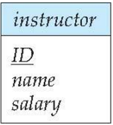
\includegraphics[width=0.45\textwidth]{../Lecture 4.4_artifacts/image_000006_bc16005a709ae01143e3342e1bc7e442c2d60be95344bd170457d511edd4a31a.png}
        \hfill
        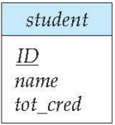
\includegraphics[width=0.45\textwidth]{../Lecture 4.4_artifacts/image_000007_443fae0583b8b7c9ed48456031cc0c4fb9e4aff544e4b91a9d80fc2bbf4176fd.png}
    \end{center}
\end{frame}

\begin{frame}{Relationship Sets}
    \begin{itemize}
        \item Diamonds represent relationship sets.
    \end{itemize}
    \begin{center}
        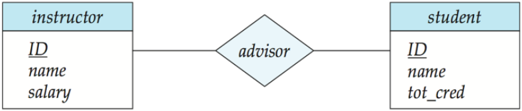
\includegraphics[height=0.7\textheight]{../Lecture 4.4_artifacts/image_000009_83b3032fcbce071acbcb3e8b9f8c7579c8f444489fece4e132d300b5e82fd68e.png}
    \end{center}
\end{frame}

\begin{frame}{Relationship Sets with Attributes}
    \begin{center}
        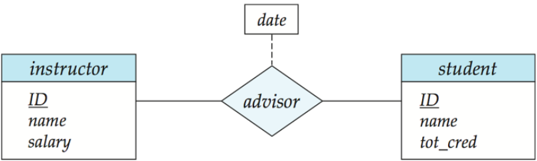
\includegraphics[width=0.8\textwidth]{../Lecture 4.4_artifacts/image_000011_ea32834193cb9b67e0fc26932e9720843839d59ed3fa8901685f6af68d47a9c0.png}
    \end{center}
\end{frame}

\begin{frame}{Roles}
    \begin{itemize}
        \item Entity sets of a relationship need not be distinct Each occurrence of an entity set plays a 'role' in the relationship
        \item The labels 'course id' and 'prereq id' are called \textbf{roles}.
    \end{itemize}
    \begin{center}
        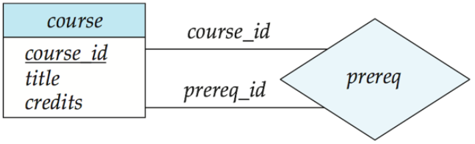
\includegraphics[width=0.6\textwidth]{../Lecture 4.4_artifacts/image_000013_7c58554f432ad0c938688ad17c19de467b3ea82a13b6d869b82adaddac21348b.png}
    \end{center}
\end{frame}

\begin{frame}{Cardinality Constraints}
    \begin{itemize}
        \item We express cardinality constraints by drawing either a directed line ($\rightarrow$), signifying 'one,' or an undirected line (--), signifying 'many,' between the relationship set and the entity set.
        \item \textbf{One-to-one relationship between an instructor and a student}:
        \begin{itemize}
            \item A student is associated with at most one instructor via the relationship advisor
            \item An instructor is associated with at most one student via the relationship advisor
        \end{itemize}
    \end{itemize}
    \begin{center}
        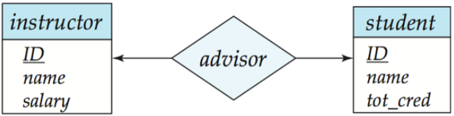
\includegraphics[width=0.8\textwidth]{../Lecture 4.4_artifacts/image_000015_507a1e843a4e0b42df9e8f6be35d49bacab575e5929b23dcc41fc9d311defde3.png}
    \end{center}
\end{frame}

\begin{frame}{One-to-Many Relationship}
    \begin{itemize}
        \item \textbf{one-to-many relationship between an instructor and a student}
        \item an instructor is associated with several (including 0) students via advisor
        \item a student is associated with at most one instructor via advisor
    \end{itemize}
    \begin{center}
        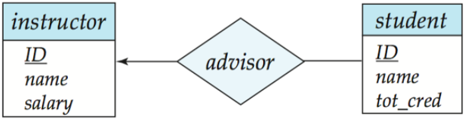
\includegraphics[width=0.8\textwidth]{../Lecture 4.4_artifacts/image_000017_b904c0e2f2b42b6e9cc2b754c50b8af4ffbe590b03d29ac4c3365b8915520ef4.png}
    \end{center}
\end{frame}

\begin{frame}{Many-to-One Relationships}
    \begin{itemize}
        \item \textbf{many-to-one relationship between a student and an instructor}
        \item an instructor is associated with at most one student via advisor
        \item a student is associated with several (including 0) instructors via advisor
    \end{itemize}
    \begin{center}
        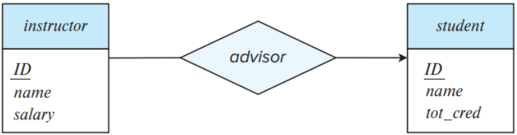
\includegraphics[width=0.8\textwidth]{../Lecture 4.4_artifacts/image_000019_e2af5a6e64b32c4f80032148b0b517faf1769596117ae7f38c8f96520f3f465d.png}
    \end{center}
\end{frame}

\begin{frame}{Many-to-Many Relationship}
    \begin{itemize}
        \item An instructor is associated with several (possibly 0) students via advisor
        \item A student is associated with several (possibly 0) instructors via advisor
    \end{itemize}
    \begin{center}
        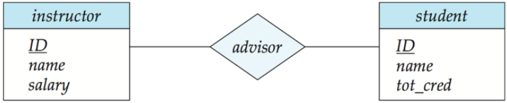
\includegraphics[width=0.8\textwidth]{../Lecture 4.4_artifacts/image_000021_d06af06551d3668aee87663f107e657c03d244e06f3aa5c7e6064030ff4859aa.png}
    \end{center}
\end{frame}

\begin{frame}{Total and Partial Participation}
    \begin{itemize}
        \item \textbf{Total participation} (indicated by double line): every entity in the entity set participates in at least one relationship in the relationship set
        \begin{itemize}
            \item participation of student in advisor relation is total
            \item every student must have an associated instructor
        \end{itemize}
        \item \textbf{Partial participation}: some entities may not participate in any relationship in the relationship set
        \begin{itemize}
            \item Example: participation of instructor in advisor is partial
        \end{itemize}
    \end{itemize}
    \begin{center}
        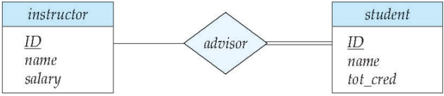
\includegraphics[width=0.8\textwidth]{../Lecture 4.4_artifacts/image_000023_6009e53301b15d60aacba843ab946adc26c5014396250447df57a8f51985808c.png}
    \end{center}
\end{frame}

\begin{frame}{Notation for Expressing More Complex Constraints}
    \begin{itemize}
        \item A line may have an associated minimum and maximum cardinality, shown in the form $l..h$, where $l$ is the minimum and $h$ the maximum cardinality
        \item A minimum value of 1 indicates total participation.
        \item A maximum value of 1 indicates that the entity participates in at most one relationship
        \item A maximum value of * indicates no limit.
    \end{itemize}
    \begin{center}
        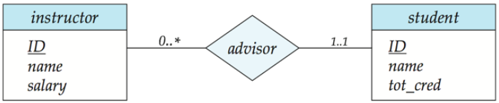
\includegraphics[width=0.8\textwidth]{../Lecture 4.4_artifacts/image_000025_aceea2eed108b6fe494f36e1658994d48f045f106d523670050ee9c423cf40be.png}
    \end{center}
\end{frame}

\begin{frame}{Notation to Express Entity with Complex Attributes}
    \begin{center}
        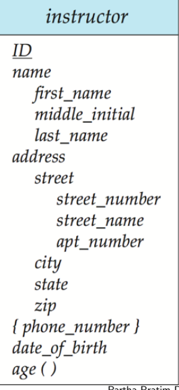
\includegraphics[width=0.45\textwidth]{../Lecture 4.4_artifacts/image_000027_e23ba19043ee6124be4c714bbe8040edd4bbb5c1dc5896a1951fd5b1d9798e58.png}
    \end{center}
\end{frame}

\begin{frame}{Expressing Weak Entity Sets}
    \begin{itemize}
        \item In ER diagrams, a weak entity set is depicted via a double rectangle
        \item We underline the discriminator of a weak entity set with a dashed line
        \item The relationship set connecting the weak entity set to the identifying strong entity set is depicted by a double diamond
        \item Primary key for section - (course\_id, sec\_id, semester, year)
    \end{itemize}
    \begin{center}
        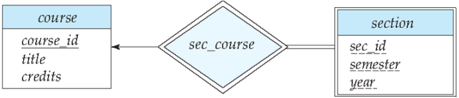
\includegraphics[width=0.6\textwidth]{../Lecture 4.4_artifacts/image_000029_bb757d7416f681cd8b8eaf8a65b4d026dd1ba70539c0b33a01dd8f8a9202eaa8.png}
    \end{center}
\end{frame}

\begin{frame}{ER Diagram for a University Enterprise}
    \begin{center}
        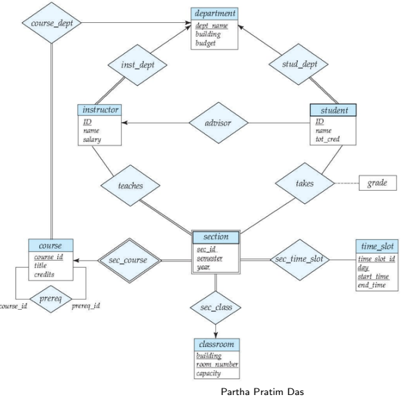
\includegraphics[height=0.8\textheight]{../Lecture 4.4_artifacts/image_000031_546762c22da1d9377e1cb5cc2e393ae96fa8a0b9785846b1b88fae1b43506797.png}
    \end{center}
\end{frame}

\section{ER Model to Relational Schema}
\begin{frame}
  \vfill
  \centering
  \begin{beamercolorbox}[sep=8pt,center,shadow=true,rounded=true]{title}
    \usebeamerfont{title}ER Model to Relational Schema\par%
  \end{beamercolorbox}
  \vfill
\end{frame}

\begin{frame}{Reduction to Relation Schema}
    \begin{itemize}
        \item Entity sets and relationship sets can be expressed uniformly as relation schemas that represent the contents of the database
        \item A database which conforms to an ER diagram can be represented by a collection of schemas
        \item For each entity set and relationship set there is a unique schema that is assigned the name of the corresponding entity set or relationship set
        \item Each schema has a number of columns (generally corresponding to attributes), which have unique names
    \end{itemize}
\end{frame}

\begin{frame}{Representing Entity Sets}
    \begin{itemize}
        \item A strong entity set reduces to a schema with the same attributes
        \begin{itemize}
            \item \texttt{student(ID, name, tot\_cred)}
        \end{itemize}
        \item A weak entity set becomes a table that includes a column for the primary key of the identifying strong entity set
        \begin{itemize}
            \item \texttt{section(course\_id, sec\_id, sem, year)}
        \end{itemize}
    \end{itemize}
    \begin{center}
        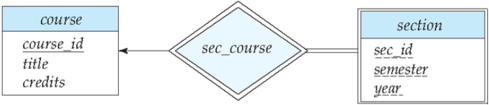
\includegraphics[width=0.45\textwidth]{../Lecture 4.4_artifacts/image_000037_93c9c824b8dcfe9fad0a59ba6498bdf79cefbdac41a866fad785fcb47377530d.png}
    \end{center}
\end{frame}

\begin{frame}{Representing Relationship Sets}
    \begin{itemize}
        \item A many-to-many relationship set is represented as a schema with attributes for the primary keys of the two participating entity sets, and any descriptive attributes of the relationship set.
        \item Example: schema for relationship set advisor
        \begin{itemize}
            \item \texttt{advisor = (s\_id, i\_id)}
        \end{itemize}
    \end{itemize}
    \begin{center}
        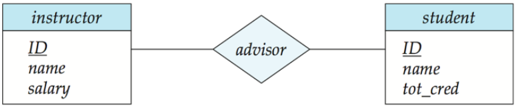
\includegraphics[width=0.45\textwidth]{../Lecture 4.4_artifacts/image_000039_6a66aae883380233f465ef450274060b650259effdee9b8d31ec1794deace3af.png}
    \end{center}
\end{frame}

\begin{frame}{Representation of Entity Sets with Composite Attributes}
    \begin{itemize}
        \item Composite attributes are flattened out by creating a separate attribute for each component attribute
        \item Example: given entity set \texttt{instructor} with composite attribute \texttt{name} with component attributes \texttt{first\_name} and \texttt{last\_name} the schema corresponding to the entity set has two attributes \texttt{name\_first\_name} and \texttt{name\_last\_name}
        \begin{itemize}
            \item Prefix omitted if there is no ambiguity (\texttt{name\_first\_name} could be \texttt{first\_name})
        \end{itemize}
        \item Ignoring multivalued attributes, extended \texttt{instructor} schema is
        \begin{itemize}
            \item \texttt{instructor(ID, first\_name, middle\_initial, last\_name, street\_number, street\_name, apt\_number, city, state, zip\_code, date\_of\_birth)}
        \end{itemize}
    \end{itemize}
    \begin{center}
        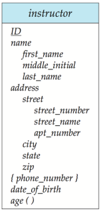
\includegraphics[width=0.45\textwidth]{../Lecture 4.4_artifacts/image_000041_1b0f12d36836debccd60e892dafb2b089ef648710adbaab7eba3499e6ed505c2.png}
    \end{center}
\end{frame}

\begin{frame}{Representation of Entity Sets with Multivalued Attributes}
    \begin{itemize}
        \item A multivalued attribute $M$ of an entity $E$ is represented by a separate schema $E_M$
        \item Schema $E_M$ has attributes corresponding to the primary key of $E$ and an attribute corresponding to multivalued attribute $M$
        \item Example: Multivalued attribute \texttt{phone\_number} of \texttt{instructor} is represented by a schema: \texttt{inst\_phone = (ID, phone\_number)}
        \item Each value of the multivalued attribute maps to a separate tuple of the relation on schema $E_M$
        \item For example, an \texttt{instructor} entity with primary key 22222 and phone numbers 456-7890 and 123-4567 maps to two tuples: (22222, 456-7890) and (22222, 123-4567)
    \end{itemize}
\end{frame}

\begin{frame}{Redundancy of Schema}
    \begin{itemize}
        \item Many-to-one and one-to-many relationship sets that are total on the many-side can be represented by adding an extra attribute to the 'many' side, containing the primary key of the 'one' side
        \item Example: Instead of creating a schema for relationship set \texttt{inst\_dept}, add an attribute \texttt{dept\_name} to the schema arising from entity set \texttt{instructor}
    \end{itemize}
    \begin{center}
        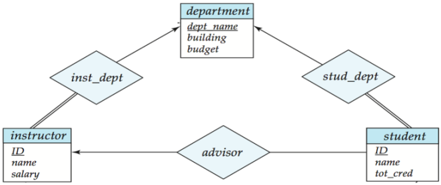
\includegraphics[width=0.45\textwidth]{../Lecture 4.4_artifacts/image_000044_4024897b11e94cfb0f653b3e23d3e87eebe2d0c5c14f9bd4cc4d9cedef4949d8.png}
    \end{center}
\end{frame}

\begin{frame}{Redundancy of Schema (2)}
    \begin{itemize}
        \item For one-to-one relationship sets, either side can be chosen to act as the 'many' side
        \item That is, an extra attribute can be added to either of the tables corresponding to the two entity sets
        \item If participation is partial on the 'many' side, replacing a schema by an extra attribute in the schema corresponding to the 'many' side could result in null values
    \end{itemize}
\end{frame}

\begin{frame}{Redundancy of Schema (3)}
    \begin{itemize}
        \item The schema corresponding to a relationship set linking a weak entity set to its identifying strong entity set is redundant.
        \item Example: The \texttt{section} schema already contains the attributes that would appear in the \texttt{sec\_course} schema
    \end{itemize}
    \begin{center}
        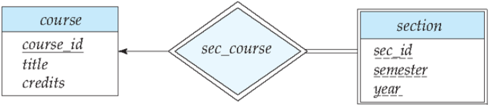
\includegraphics[width=0.6\textwidth]{../Lecture 4.4_artifacts/image_000048_b3bd085c01161ccfa937a5f3d7699c1c92943aeb0a346080fb2c961ede5df4f3.png}
    \end{center}
\end{frame}

\begin{frame}{Module Summary}
    \begin{itemize}
        \item Illustrated ER Diagram notation for ER Models
        \item Discussed translation of ER Models to Relational Schema
    \end{itemize}
    \vspace{2em}
    \begin{center}
    \small \textit{Slides used in this presentation are borrowed from \url{http://db-book.com/} with kind permission of the authors.} \\
    \small \textit{Edited and new slides are marked with 'PPD'.}
    \end{center}
\end{frame}

\end{document}
